\section*{Experimentación con httping}

\noindent El primer paso para este experimento es escoger los destinos en otros continentes. Los destinos seleccionados son:

\begin{description}
    \item[America] - http://www.iztapalapa.uam.mx/
	\item[Australia] - https://sydney.edu.au/
	\item[Europa] - https://universidadeuropea.com/
\end{description}

\begin{lstlisting}[language=Bash, caption=Pings con 300 muestras guardando la salida, label=lst:pings]
	httping -c 300 http://www.iztapalapa.uam.mx/ > uam_full.dat
	httping -c 300 https://sydney.edu.au/ > australia_full.dat
	httping -c 300 https://universidadeuropea.com/ > espana_full.dat
\end{lstlisting}

\noindent Ahora que tenemos los archivos con toda la informaci\'on de los ping es necesario extraer solo el valor num\'erico de estos. Para ello usaremos el script AWK visto en la \emph{Figura }\ref{fig:scriptAWK}. Con la informaci\'on necesaria en archivos individuales sigue trazar por separado las tres gr\'aficas obtenidas. A continuaci\'on se muestran las tres gr\'aficas y las instrucciones en Octave para generarlas

\newpage

\begin{figure}[H] 
    \centering 
    \begin{lstlisting}[frame=single, breaklines=true, basicstyle=\footnotesize\ttfamily, breakatwhitespace=false, columns=flexible, tabsize=2, showstringspaces=false, language=Octave] 
        load uam_RTT.dat 
        plot(uam_RTT, '--*', 'Color', 'k', 'LineWidth', 0.5, 'MarkerSize', 8) 
        grid on 
        xlabel ('Vuelta de transmision') 
        ylabel ('Ping [ms]') 
        title('Ping http://www.iztapalapa.uam.mx/') 
        print -dpng "trazaUam.png" 
    \end{lstlisting} 
    \caption{Instrucciones para trazar la gr\'afica} 
    \label{fig:uamOctave} 
\end{figure}

\begin{figure}[H]
	\centering
	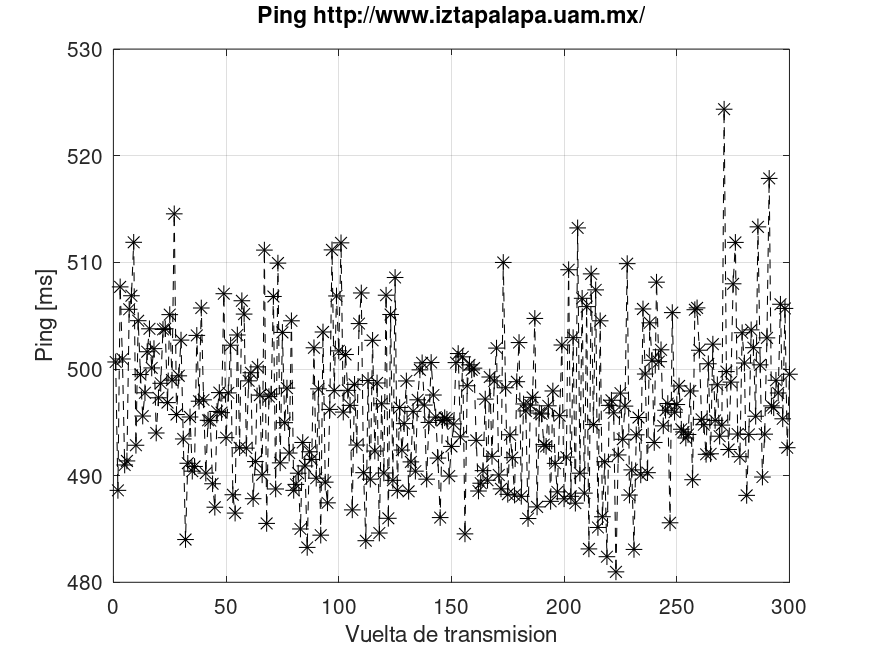
\includegraphics[width=0.90\textwidth]{img/trazaUam.png}
	\caption{Gr\'afica de los datos del ping a http://www.iztapalapa.uam.mx/}
	\label{fig:uamGraph}
\end{figure}

\newpage

\begin{figure}[H] 
    \centering 
    \begin{lstlisting}[frame=single, breaklines=true, basicstyle=\footnotesize\ttfamily, breakatwhitespace=false, columns=flexible, tabsize=2, showstringspaces=false, language=Octave] 
        load australia_RTT.dat 
        plot(australia_RTT, '--*', 'Color', 'b', 'LineWidth', 0.5, 'MarkerSize', 8) 
        grid on 
        xlabel ('Vuelta de transmision') 
        ylabel ('Ping [ms]') 
        title('Ping https://sydney.edu.au/') 
        print -dpng "trazaAustralia.png" 
    \end{lstlisting} 
    \caption{Instrucciones para trazar la gr\'afica} 
    \label{fig:australiaOctave} 
\end{figure}

\begin{figure}[H]
	\centering
	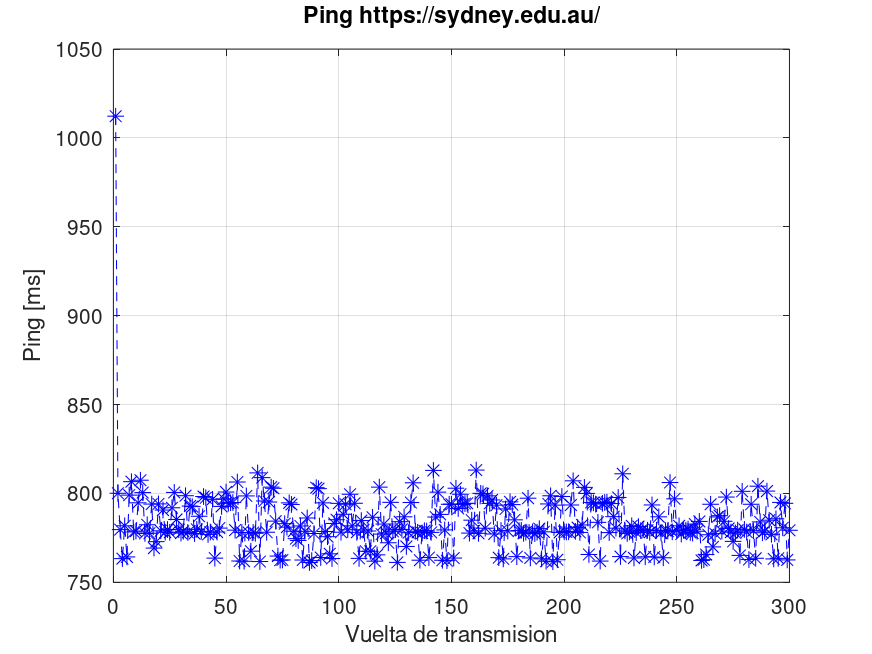
\includegraphics[width=0.90\textwidth]{img/trazaAustralia.png}
	\caption{Gr\'afica de los datos del ping a https://sydney.edu.au/}
	\label{fig:australiaGraph}
\end{figure}

\begin{figure}[H] 
    \centering 
    \begin{lstlisting}[frame=single, breaklines=true, basicstyle=\footnotesize\ttfamily, breakatwhitespace=false, columns=flexible, tabsize=2, showstringspaces=false, language=Octave] 
        load espana_RTT.dat 
        plot(espana_RTT, '--*', 'Color', 'r', 'LineWidth', 0.5, 'MarkerSize', 8) 
        grid on 
        xlabel ('Vuelta de transmision') 
        ylabel ('Ping [ms]') 
        title('Ping https://universidadeuropea.com/') 
        print -dpng "trazaEspana.png" 
    \end{lstlisting} 
    \caption{Instrucciones para trazar la gr\'afica} 
    \label{fig:espanaOctave} 
\end{figure}

\begin{figure}[H]
	\centering
	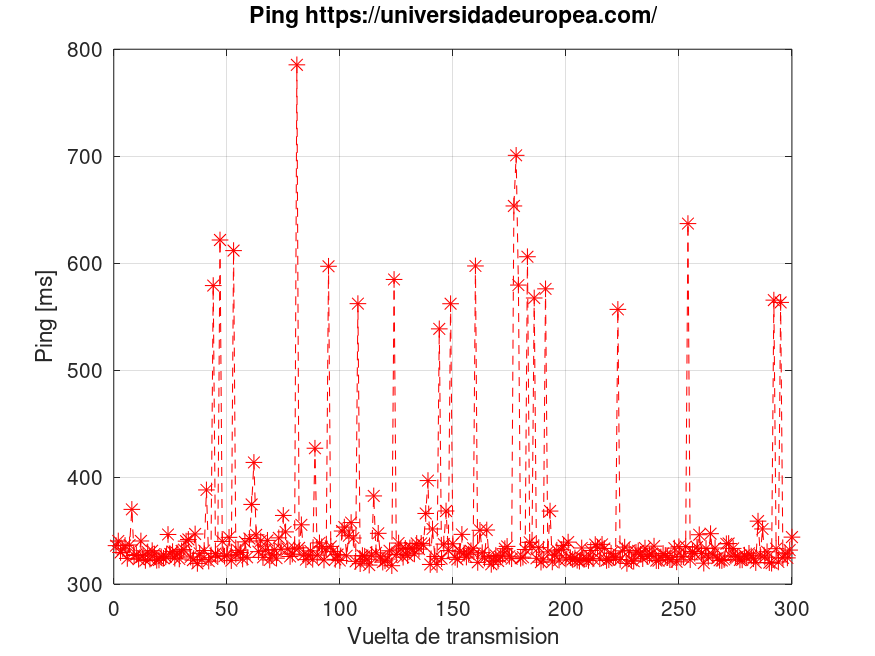
\includegraphics[width=0.90\textwidth]{img/trazaEspana.png}
	\caption{Gr\'afica de los datos del ping a https://universidadeuropea.com/}
	\label{fig:espanaGraph}
\end{figure}

\noindent Lo primero que se puede observar con este nuevo proceso la magnitud del RTT es m\'as grande que con el uso de ping. Investigando un poco sobre que mide cada herramienta se pueden considerar los siguientes puntos:

\begin{description}
    \item[Ping] - Mide principalmente el RTT para paquetes entre dos puntos.
    \item[Httping] - Mide el tiempo de ida y vuelta para solicitudes HTTP completas, incluyendo el tiempo de conexi\'on, transferencia de datos y respuesta. 
\end{description}

\noindent En general, el ping es m\'as r\'apido pero menos representativo del rendimiento real de las aplicaciones web, mientras que httping da un resultado m\'as preciso pero tarda m\'as.